\chapter{Interaction of Gammas With Matter}\label{chap:gammas}
The gamma-rays (or gammas for short) produced in nuclear processes open a window into the nucleus. The energy of these gammas are tied to nuclear energy levels, thus once measured, their study provides a pathway for isotope identification. Radioactive decay often populate excited nuclear states, resulting in gammas that, although informative, are a dominant background in rare-event searches. Understanding the ways in which gammas interact with matter is essential to the design of any experiment wishing to detect rare events. The gammas produced in the decay chains of the primordial isotopes, Th$^{232}$ and U$^{238}$ -- isotopes which are present in trace quantities in all materials on Earth -- can penetrate several centimeters of shielding or detector material. While this poses a problem to rare-event searches, the highly penetrating nature of gammas, and specifically the ability to tune this penetration depth by choosing a gamma energy, provides a rich tool for the study of detectors. This chapter provides an overview of the dominant interactions of gammas with matter and elucidates how monoenergetic gammas can be used for the study of semiconductor detectors -- a topic which will be treated in detail in Chapter~\ref{chap:scanner}.

%In contrast with alpha and beta particles, gamma-ray photons (or gammas for short) carry no charge and thus do not participate in Coulomb interactions. Therefore, they cannot be detected directly. They share this ``ghostlike'' behavior with neutrinos, a particle which can transverse light-years of dense material without interacting~\cite{close_particlebook}. However, the probability of interaction of gammas with matter is orders of magnitude higher, such that they can be fully stopped within everyday-sized objects.

To detect a gamma particle, it must transfer energy to an electron in the absorbing material. The three major energy transfer mechanisms are: the photoelectric effect, Compton scattering and pair production. The resulting free electrons ionize the material along their tracks. They can also lose energy through bremsstrahlung (braking radiation). 

\section{Photoelectric Effect}
At gamma energies below 180\,keV, the dominant interaction mechanism of gammas with matter is the photoelectric effect. A gamma with sufficient energy can be absorbed by orbital electron of an atom in an absorber. If the photon energy, $E_\text{in}$, is sufficiently high,  the electron is emitted with an energy of: 
\begin{equation}
	E_e = E_\text{in} - E_b~, 
	\label{eq:photoelectric_intro}
\end{equation}
where $E_b$ is the binding energy of the orbital electron. At energies $E_e$, the resulting \textit{photoelectron} has a small range and ionizes locally. The photoelectron creates a vacancy in the absorber atom which is quickly filled by rearrangement of the orbital electrons or by a free electron. Thus, besides the energetic photoelectron, an energy of $E_b$ is also released into the absorber medium. This energy can take the form of a characteristic X-ray or an Auger electron. Given the range of these particles, $E_b$ will also be deposited in a small volume around the original interaction site.

The probability of the photoelectric absorption is greatly enhanced by the number of protons, $Z$, of the absorbing atom. This probability is roughly proportional to $Z^n/E_\text{in}^{3.5}$, where $n$ varies between 4 and 5 depending on $E_{in}$~\cite{knoll}.

\section{Compton Scattering}
The energy of the incident gamma can also be partially transferred to an electron in the absorber via the Compton effect. In this scenario, the gamma scatters off an electron and deviates from its original trajectory by an angle $\theta$. The energy of the scattered gamma, $E_\text{out}$, is
\begin{equation}
	E_\text{out} = \frac{E_\text{in}}{1 + \frac{E_\text{in}}{m_ec^2}(1 - \cos\theta)}~,
	\label{eq:compton_intro}
\end{equation}
where $m_e$ is the mass of the electron~\cite{compton}. The electron recoils with an energy of $E_e = E_\text{in} - E_\text{out}$. As can be seen by manipulation of Eq.~\ref{eq:compton_intro}, while no minimum energy transfer is required, the maximum energy transfer occurs at $\theta = \pi$. This energy is referred to as the ``Compton edge''.

The Compton effect dominates when the incident gamma energy is between 180\,keV and 8\,MeV. The probability of Compton scattering depends on the number of electrons in the absorber and is therefore proportional to $Z$. While, the scattering angle, $\theta$ can take any value, not all angles are equiprobable. This relation is given by the differential scattering cross-section, $d\sigma/d\Omega$, predicted by the Klein-Nishina formula:
\begin{equation}
	\frac{d\sigma}{d\Omega} = Zr_0^2\left(\frac{1}{1+\epsilon_\text{in}(1 - \cos\theta)}\right)^2 \left(\frac{1 + \cos^2\theta}{2}\right) \left(1 + \frac{\epsilon_\text{in}^2(1-\cos\theta)^2}{(1+\cos^2\theta)\left[1+\epsilon_\text{in}(1-\cos\theta)\right]}\right)~,
	\label{eq:klein-nishina}
\end{equation}
where $\epsilon_\text{in} \equiv E_\text{in}/m_ec^2$ and $r_0$ is the classical electron radius~\cite{klein-nishina}. This cross-section is plotted for all energies between 1\,keV and 10\,MeV in Fig.~\ref{fig:klein-nishina}. Note that the probability of forward scattering is enhanced at higher energies. 

\begin{figure}[htb]
	\centering
	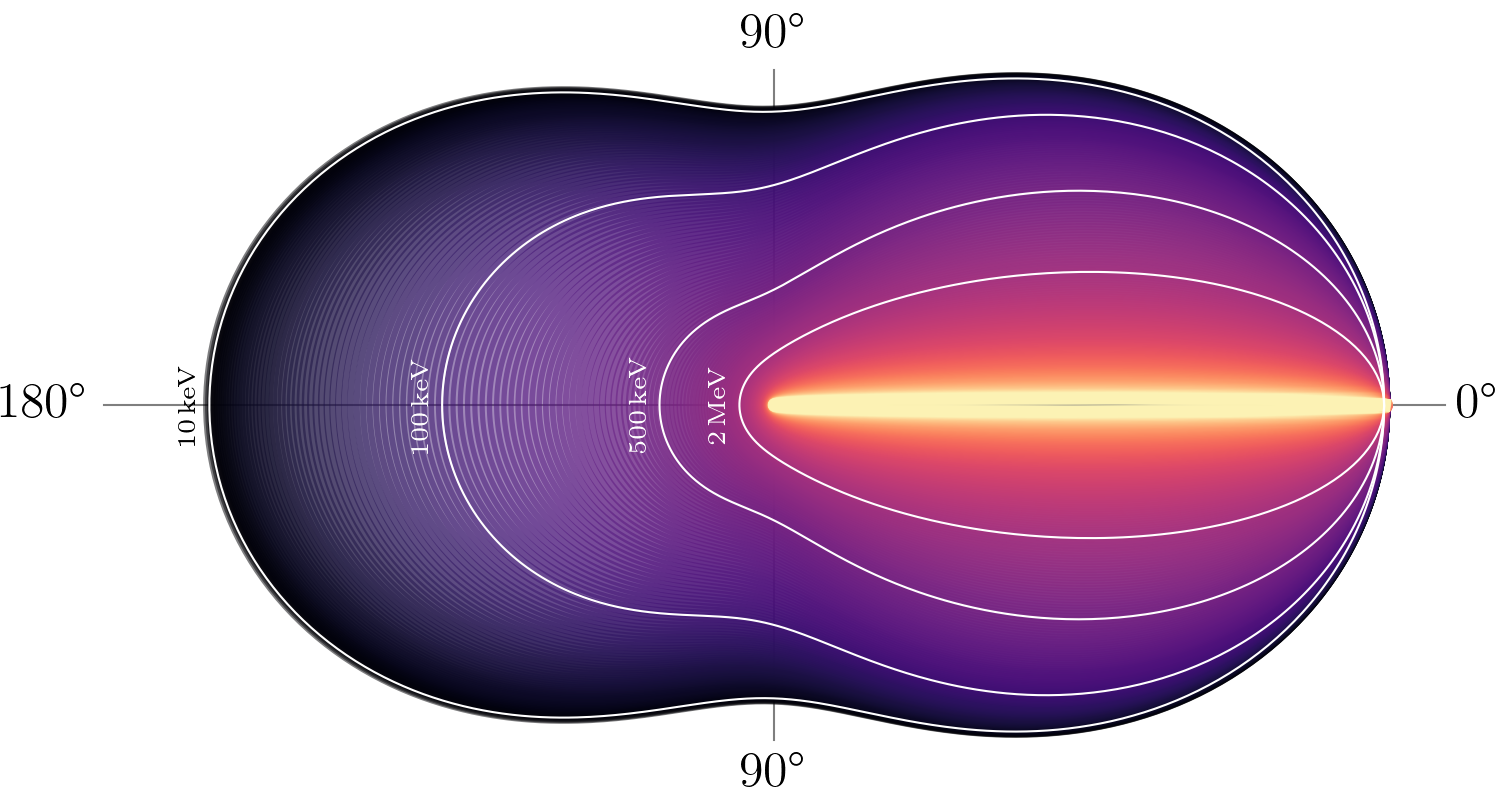
\includegraphics[width=5in]{figs/gammas/klein_nishina_width_5in.png}
	\caption{Klein-Nishina differential scattering cross-section for incident gamma energies between 1\,keV and 10\,MeV. Brighter colors indicate higher incident gamma energy. Four energy levels are marked in white.}
	\label{fig:klein-nishina}
\end{figure}

\section{Pair Production}
At gamma energies above $2m_ec^2 = 1.02$\,MeV, pair-production becomes possible. However, the probability of pair production is subdominant until incident gamma energies of 8\,MeV. In the presence of an electric field, the incident gamma can resolve into an electron-positron pair~\cite{pair_production}. The surplus gamma energy, is shared by the electron and positron in the form of kinetic energy:
\begin{equation}
	E_e + E_{e^+} = E_\text{in} - 2m_ec^2~.
\label{eq:pairproduction_intro}
\end{equation}
The electron and positron will gradually lose their energy in the absorber medium. Additionally, the positron will annihilate in the medium, leading to the production of two 511\,keV gammas (annihilation gammas). Compared to the characteristic X-rays produced in photoelectric absorption, these annihilation gammas have far longer attenuation lengths and lead to significant consequences in gamma-ray spectroscopy.  

\section{Attenuation Length}
\begin{figure}[htb]
	\centering
	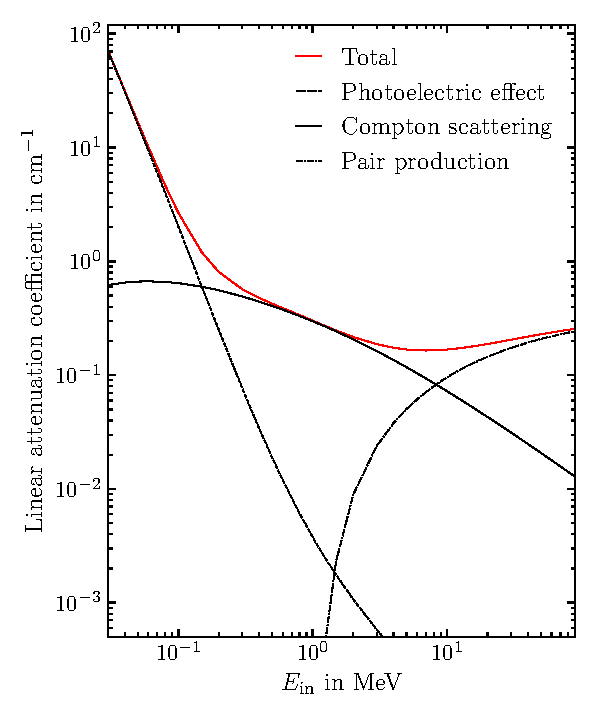
\includegraphics{figs/gammas/linear_attenuation_ge_width_4in.pdf}
	\caption{Total linear absorption coefficient (not including coherent scattering) in Ge. The contributions from the photoelectric effect, Compton scattering and pair production are shown. Data points are sourced from Ref.~\cite{NIST}.}
	\label{fig:attenuation}
\end{figure}
Gamma-ray intensity decreases exponentially as gammas transverse an absorber. Depending on the energy, gammas will undergo photoelectric absorption, Compton scattering, or if energetically allowed, pair production, exponentially attenuating the ray's intensity, $I_0$, to $I$ in a path of length $l$:
\begin{equation}
	I = I_0e^{-\mu l}~,
\label{eq:attenuation_length}
\end{equation}
where $\mu$ is the total linear attenuation coefficient~\cite{knoll}. It includes contributions from the three interaction mechanisms described above: $\mu = \mu_\text{Photoelectric} + \mu_\text{Comton} + \mu_\text{Pair}$. The exact contribution from each mechanism is plotted for incident gamma energies between 30\,keV and 90\,MeV in Fig.~\ref{fig:attenuation}. The attenuation length is defined as the length over which the intensity is attenuated to $I/I_0 = 1/e$ and is numerically equal to $1/\mu$. The strong dependence of $\mu_\text{Photoelectric}$ on $1/E_\text{in}^{3.5}$ gives rise to the steep rise in attenuation length from 30\,keV to 180\,keV seen in Fig.~\ref{fig:attenuation}. In this chapter, Ge is used as an example absorber. In contrast to the photoelectric effect and Compton scattering (above 100\,keV), the probability of pair production increases with energy. Therefore, the attenuation length increases monotonically with energy until around 6\,cm in Ge at 7\,MeV~\cite{NIST} and then decreases as the probability for pair production continues to increase. 

\section{Gamma-Ray Spectroscopy}
As opposed to the optical and characteristic X-rays emitted from orbital electron transitions, nuclear energy transitions are generally orders of magnitude higher, with energies ranging from a few keV to about 10\,MeV range~\cite{knoll}. These transitions can be studied by measuring the energy of the resulting gammas.

The detection and energy estimation of gammas relies on the production of an energetic electron (or electron-positron pair) and its subsequent loss of energy in an active medium (detector). Electrons lose energy trough electromagnetic interactions with orbital electrons (and to a lesser extent nuclei) along an erratic path through the medium. These collisional losses, ionize or excite atoms in the electron's path. The collection of free electrons released by ionization from the primary electron provides a mechanism for particle detection and energy estimation. Note that for an accompanying primary positron in pair production, the same principles apply. For an accurate energy estimation, many conditions have to be met. The primary electron (and positron if present) needs to be contained in the active volume of the detector. Thus, the stopping power of the detector medium is of great importance. Fig.~\ref{fig:stopping} shows the linear stopping power ($dE_e/dl$) of Ge as a function of electron energy, $E_e$. 
\begin{figure}[htb]
	\centering
	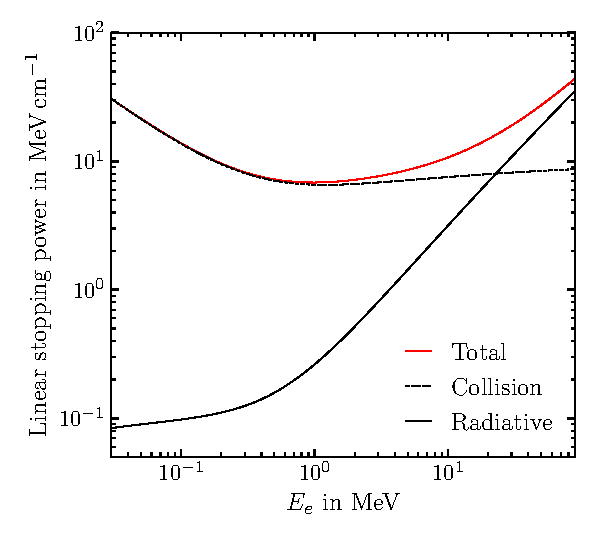
\includegraphics{figs/gammas/linear_stopping_ge_width_4in.pdf}
	\caption{Total linear stopping power of Ge and a function of electron energy, $E_e$. The contributions from collision and radiative (bremsstrahlung) effects are shown. Data points are sourced from Ref.~\cite{NIST_e}}
	\label{fig:stopping}
\end{figure}

It is clear from this relation that up to one centimeter of Ge is required to stop the energetic primary electrons produced in gamma interactions. The collision component of the linear stopping power scales with $Z$~\cite{bethe}, while the radiative component scales with $Z^2$~\cite{bremsstrahlung}. Therefore, a detector with high $Z$ will have significantly more stopping power. Meanwhile, both collision and radiative stopping power scale with the number density of the absorbing medium. Combining these facts, it is clear that detectors with dense active volumes are advantageous.  

At electron energies above 1\,MeV bremsstrahlung becomes significant. The electron looses energy through the emission of bremsstrahlung, since it is a charged particle under acceleration~\cite{bremsstrahlung,larmor}. Amongst other effects, radiative losses and the production of characteristic X-rays, provide a mechanism for energy loss, even when the primary electron is fully contained in the detector. Nevertheless, bremsstrahlung photons and the characteristic X-rays and the auger electrons produced in photoelectric absorption have very short ranges and will be contained in the cm of Ge described above. These secondary particles will undergo interactions within the medium themselves, causing a cascade of secondary electrons which will contribute to ionization and restore the lost energy of the primary interaction. It is possible that these particles escape the detector if the primary energy deposition occurs at the surface, however such effects become negligible as the volume to surface ratio increases. 

In a Ge detector with an active volume thickness around 1\,cm or above, incident monoenergetic gammas undergoing photoelectric absorption appear in the detector spectrum as a single full energy peak (FEP). In contrast, Compton scattered gammas are often energetic enough to escape the detector entirely without undergoing secondary interactions. For this reason, a Compton continuum is formed. The continuum ranges from zero to the Compton edge, which corresponds to backscatters depositing the maximum allowed energy in the detector. If only one scatter occurs in the detector the continuum takes the incident-gamma-energy-dependant form shown by Fig.~\ref{fig:compton_shapes}. This continuum can be found along with the FEP in monoenergetic gamma spectra with a gap in between corresponding to the energy of a backscattered gamma. Multiple scatters within the detector will alter the shape predicted in Fig.~\ref{fig:compton_shapes} and populate the gap between the Compton edge and FEP. If the multiple scatters culminate in a photoelectric absorption event, the full energy is contained, thus populating the FEP. The Peak-to-Compton ratio -- the ratio between the height of the FEP and that of the Compton continuum -- increases with larger detectors. 
\begin{figure}[htb]
	\centering
	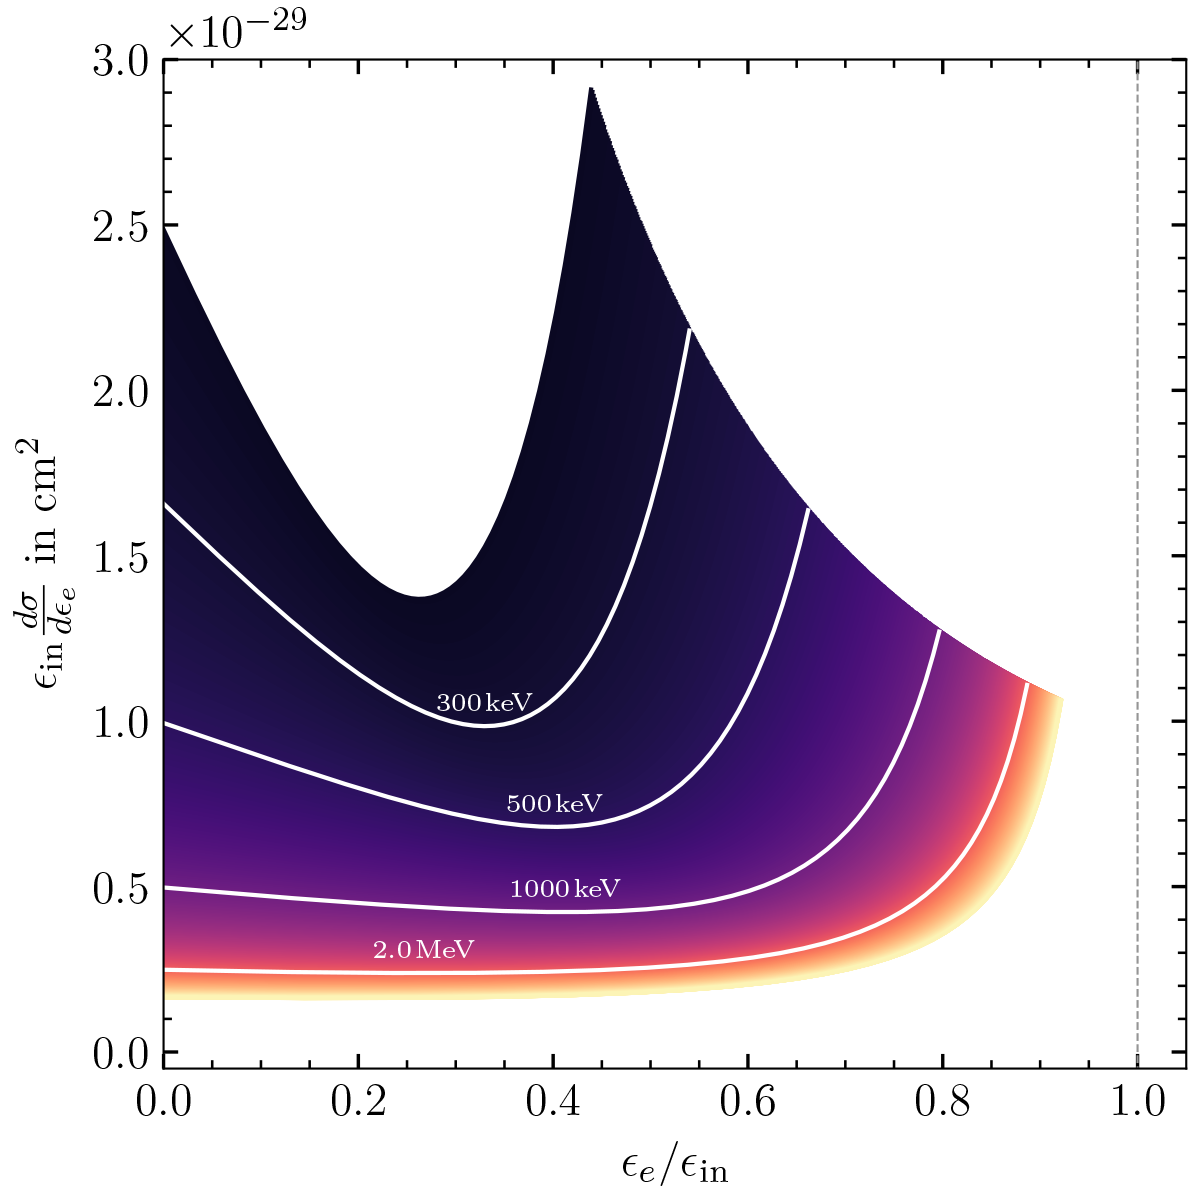
\includegraphics[width=4in]{figs/gammas/compton_shape_width_4in.png}
	\caption{Shape of the Compton continuum for incident gamma energies between 200\,keV and 3\,MeV in Ge, as calculated from its differential cross-section $\frac{d\sigma}{d\epsilon_e} = 2\pi\sin\theta\frac{d\theta}{d\epsilon_e}\frac{d\sigma}{d\Omega}$. The fist partial on the right-hand side is calculated from Eq.~\ref{eq:compton_intro} and the second is given directly by Eq.~\ref{eq:klein-nishina}. Note that $\epsilon_{e/\text{in}} = E_{e/\text{in}}/m_ec^2$. Brighter colors indicate higher incident gamma energy. Four energy levels are marked in white. A dashed gray line marks the location of the associated FEP for all energies.}
	\label{fig:compton_shapes}
\end{figure}

Pair production introduces another interesting effect in the spectrum. The energy in surplus of 1.02\,MeV is deposited in the detector by the electron and positron. However, energy was ``spent'' on the creation of the electron (and positron), which will just come to rest in the medium. The positron recovers this seemingly lost energy via its annihilation with an electron in the detector. Two back-to-back 511\,keV gammas are created. If both are contained in the detector, the event's energy will fall in the FEP. However, given the roughly 24\,mm attenuation length of 511\,keV gammas in Ge, one or both gammas can escape the detector. Two peaks form in the spectra -- the single and double escape peaks (SEP, DEP) -- each one corresponding to the escape of one or both annihilation gammas from the detector. These are found 511\,keV and 1.02\,MeV below the associated FEP. The Compton continuum, SEP, DEP associated with the 2.615\,MeV $^{208}$Tl FEP can be observed in the spectrum in Fig.~\ref{fig:spectrum_features}.
\begin{figure}[htb]
	\centering
	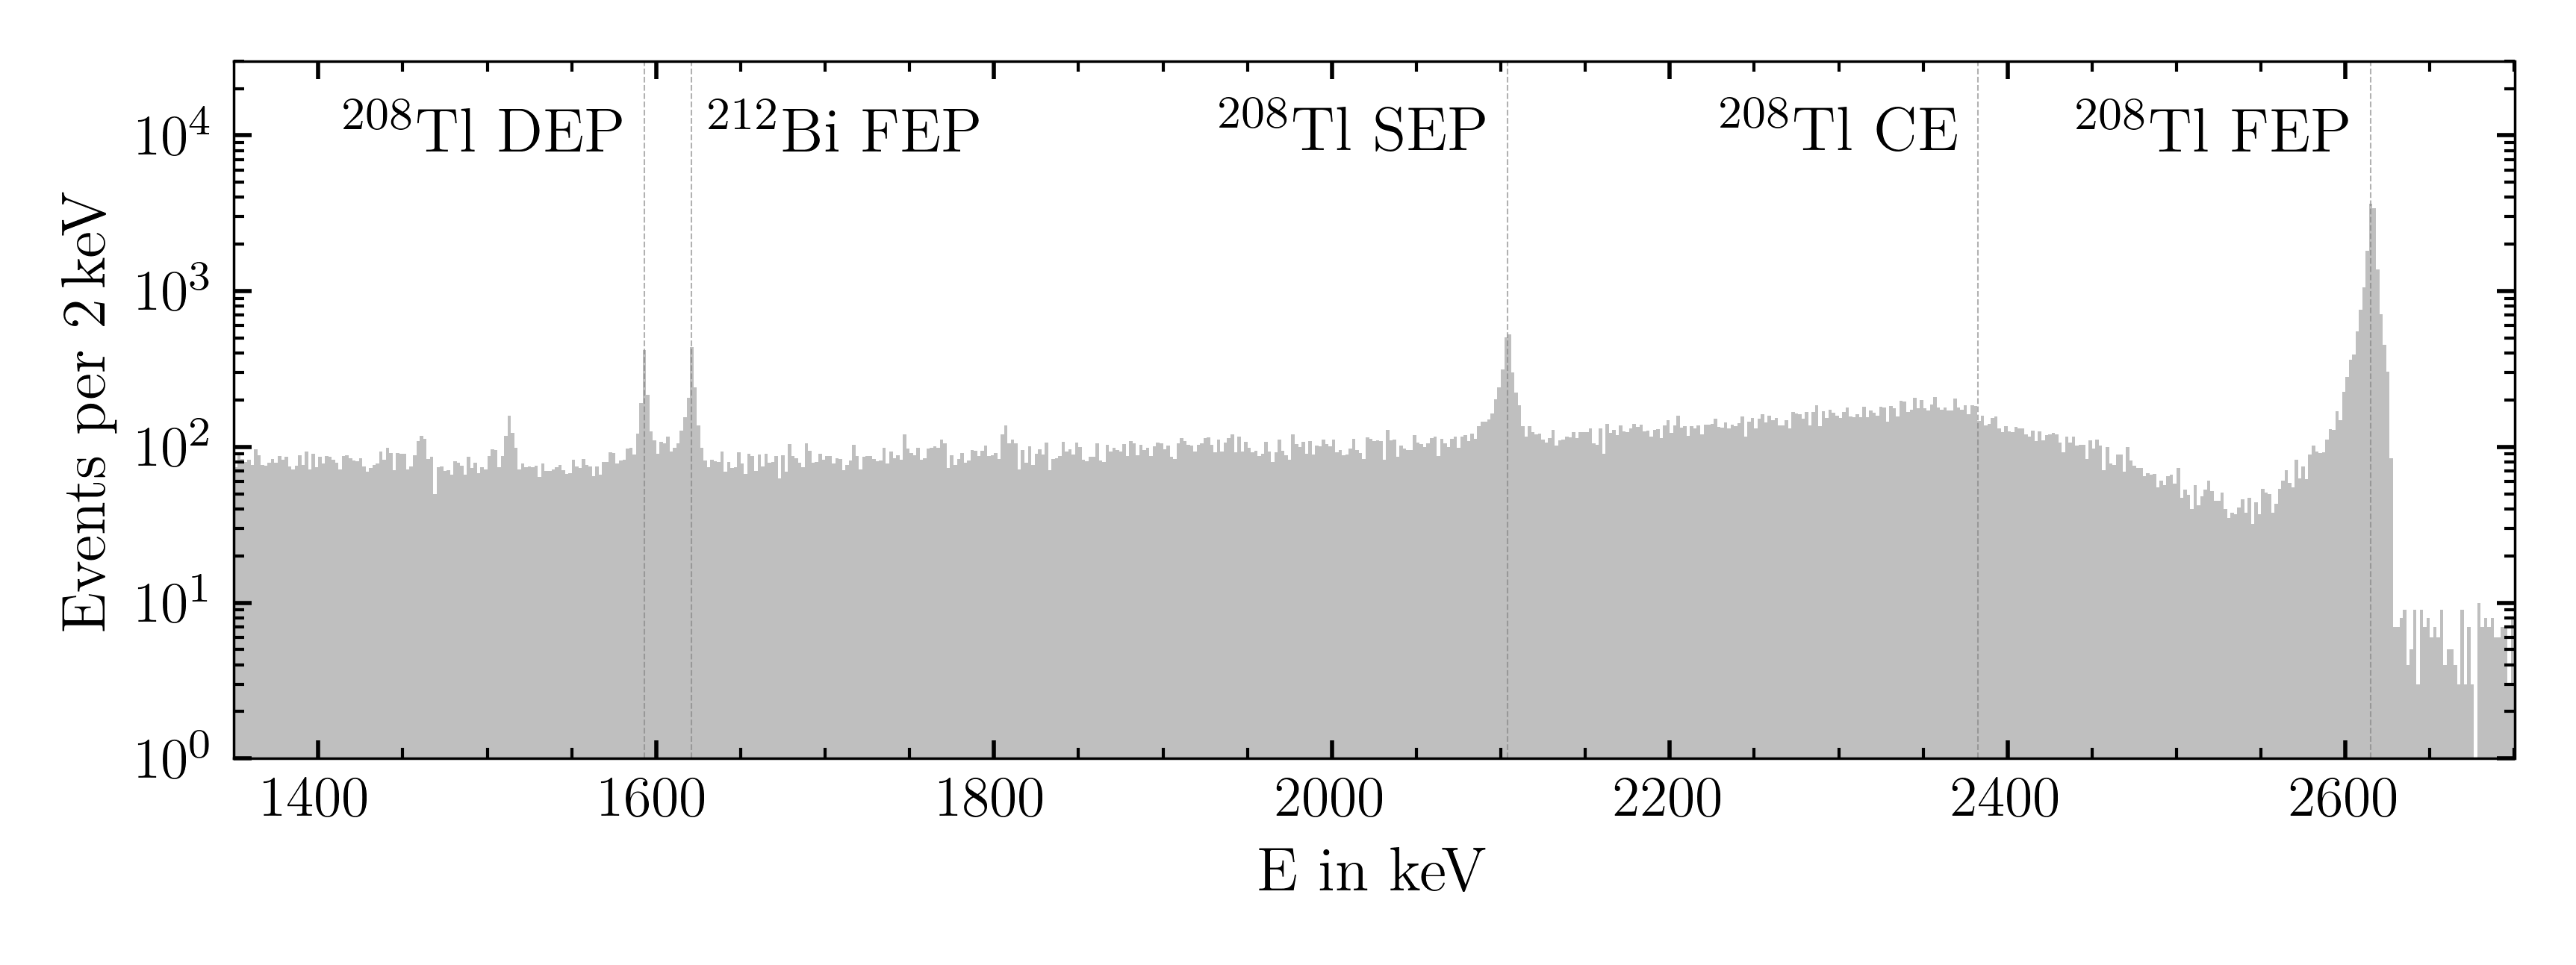
\includegraphics[width=6in]{figs/gammas/Th228_spectrum_features.png}
	\caption{Main features of a $^{228}$Th spectrum in the 1350-2700\,keV range taken with a Ge detector. The energies shown are calculated as the raw data acquisition output times a calibration constant. The full energy peak (FEP) of $^{208}$Tl and $^{212}$Bi and the single escape peak (SEP), double escape peak (DEP) and the Compton edge (CE) of $^{208}$Tl are labeled.}
	\label{fig:spectrum_features}
\end{figure}

Although a detector thickness of 1\,cm is sufficient to contain and measure the full energy of an incident gamma if it undergoes photoelectric absorption, it corresponds to roughly one attenuation length of 180\,keV gammas in Ge. Therefore, this thickness is inadequate for gamma-ray spectroscopy at higher energies, where the attenuation length grows and the Compton effect and pair production dominate. To achieve a good Peak-to-Compton ratio, much larger detectors are required.

The constraints outlined in this chapter pose a unique set of requirements for detectors suitable for gamma-ray spectroscopy. The detectors should be dense, pointing to the use of solids. Additionally, the active volume of the detector should be large enough to fully absorb gamma rays of wide-ranging energies with high probability. As will be seen in the next chapter, Ge detectors are optimal for gamma-ray spectroscopy due to their high density, moderately high $Z$, uniquely large active volume (for semiconductor detectors), and superb energy resolution.